Solve the boundary value problem $u_{xx}+4u_x+e^xu=\sin(8x)$ numerically on $[-1,1]$ with boundary
conditions $u(\pm1)=0$. To ten digits of accuracy, what is $u(0)$?\\\\

\begin{solution}\renewcommand{\qedsymbol}{}\ \\
    For this problem, we have both a first order and a second order term in our equation, so we will use
    a first and second order Chebyshev matrix. After running through the code below, we have that
    $u(0)\approx0.009597857230$ and we also get the following graph with $N=50$.

    \begin{figure}[htp]
        \centering
        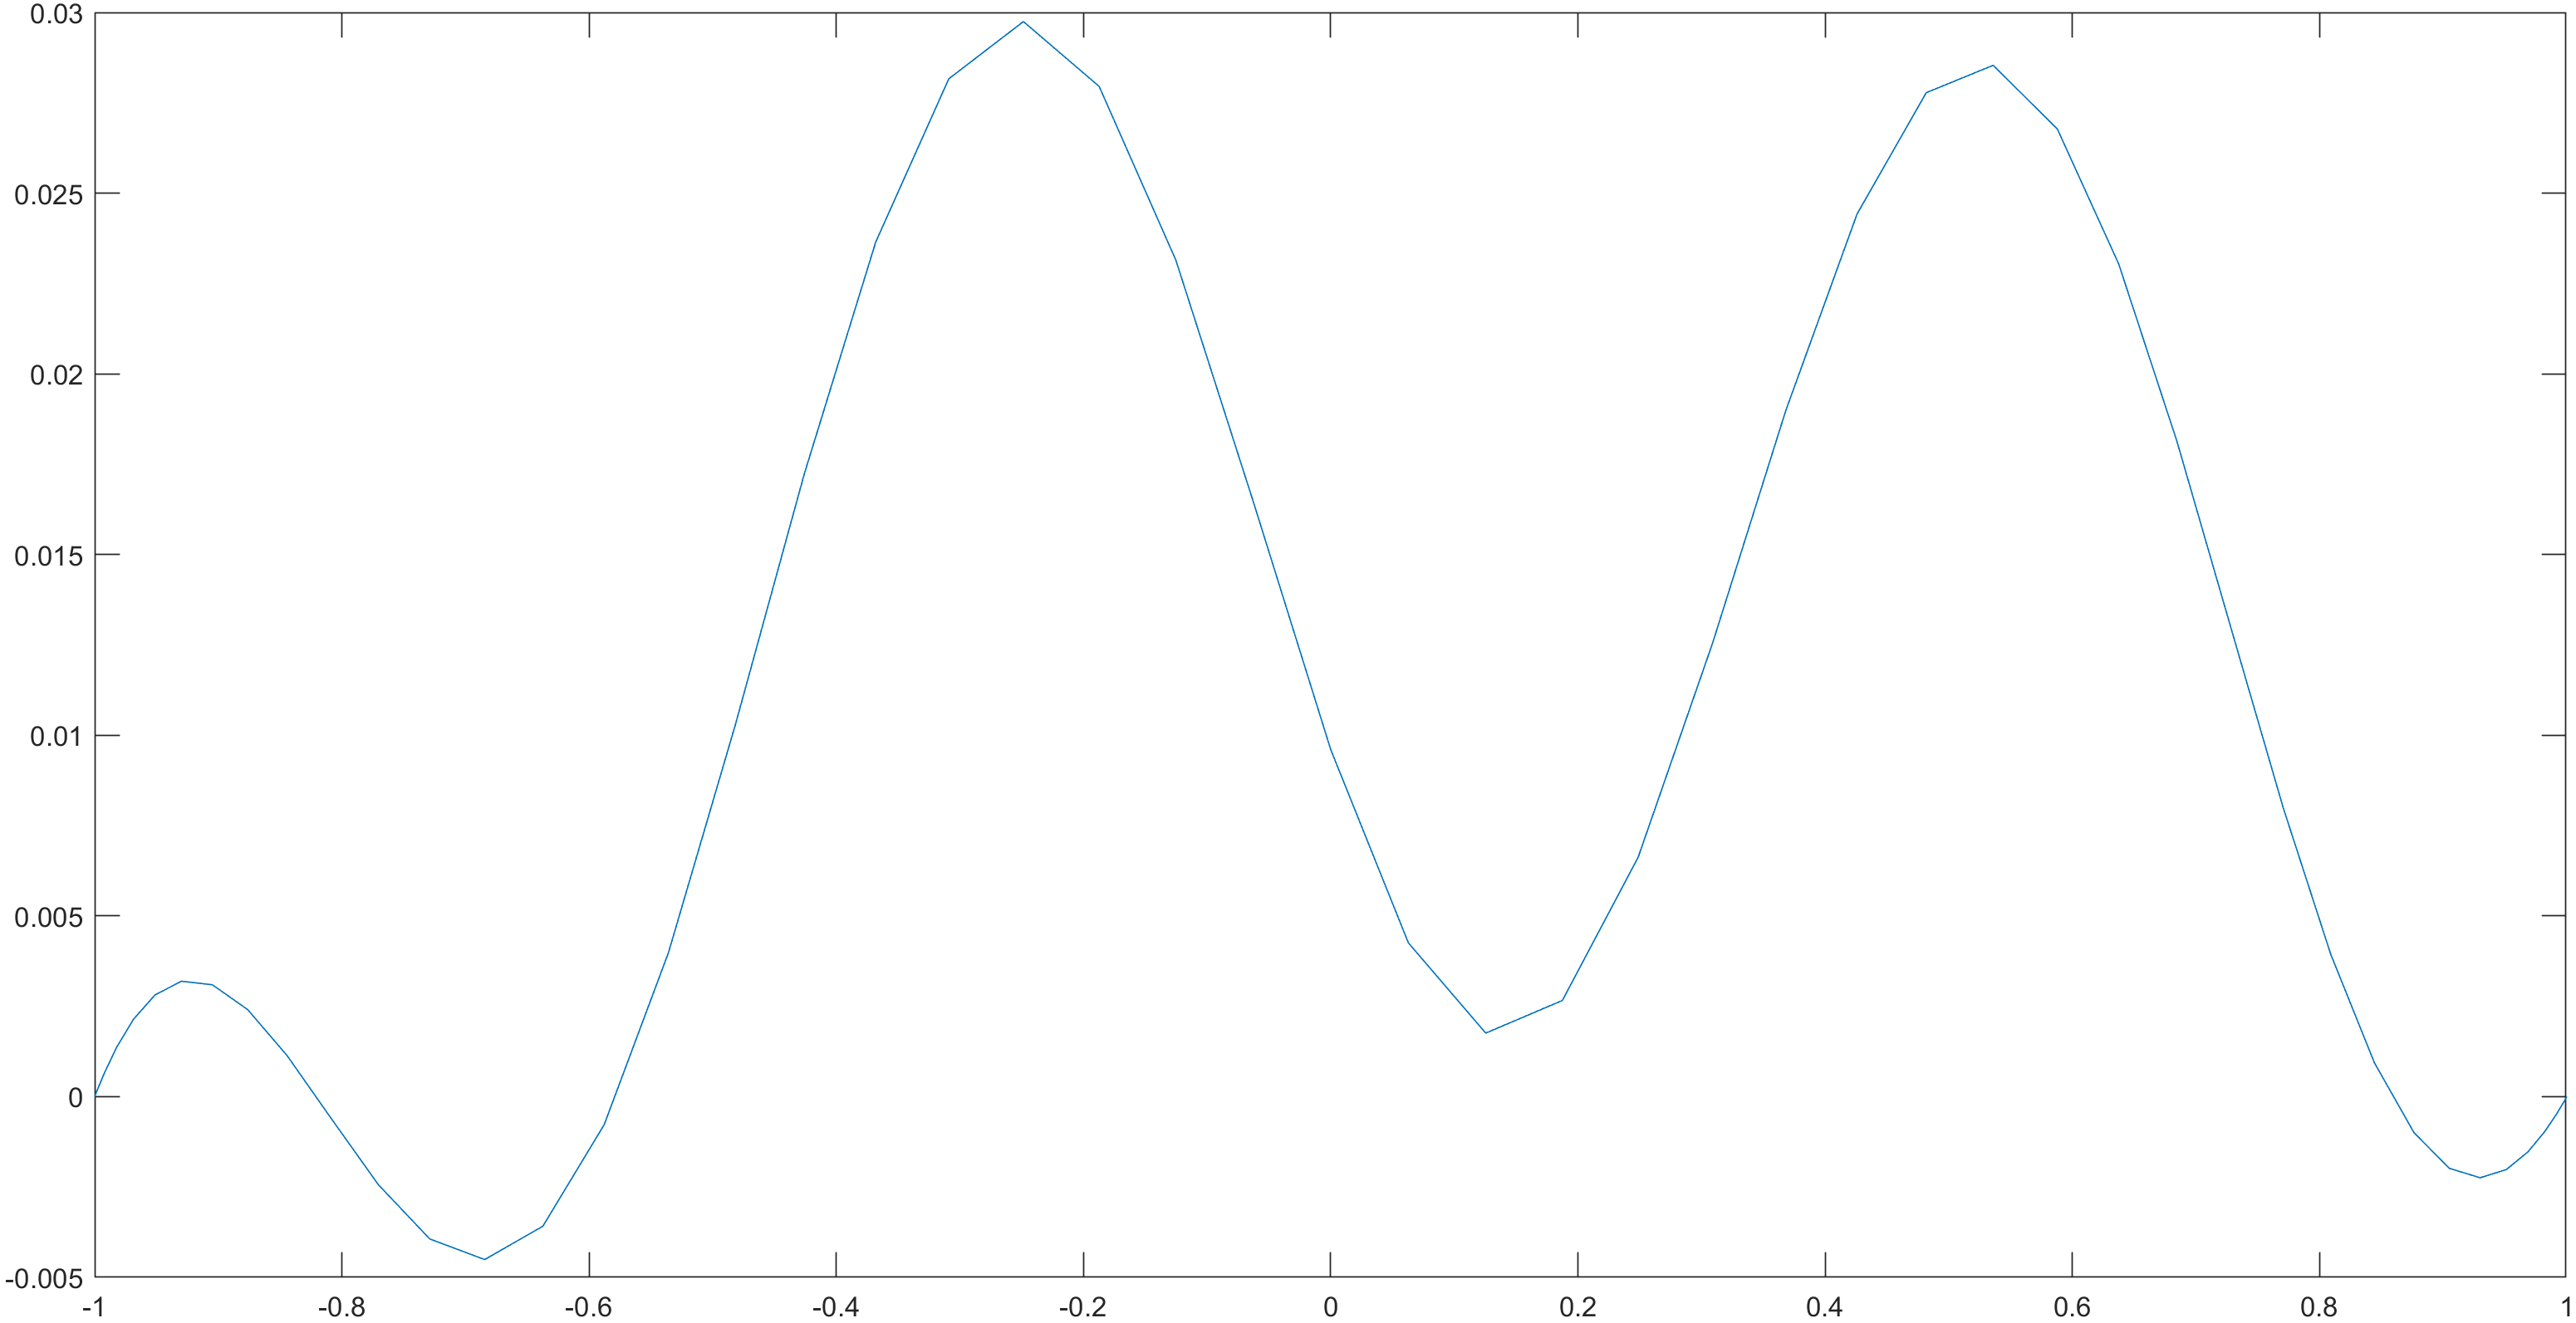
\includegraphics[scale=0.14]{7_2.PNG}
    \end{figure}

\end{solution}

\newpage
\lstinputlisting{problem7_2.m}
\newpage 